%SETTINGS
\newpage
\setcounter{page}{1}
\justifying
\noindent

%WRITING
\section{Navigation}
The first section of this paper will discuss in regards to navigation. The focused topic will be the Inertial Navigation System (INS) and Enhanced Long Range Navigation system (E-LORAN). This section will include a brief introduction, system mechanism, and real-life application for each type of navigation.\\

\subsection{Inertial Navigation System (INS)}
Inertia is the ability of any physical object to maintain its translational and rotational velocity unless external forces act upon them. Inertial navigation is self-contained navigation that is used to track body position, and orientation relative to its initial condition (point, orientation, and velocity) \cite{Woodman2007NumberNavigation}\cite{Ribbens2003AircraftInstruments}. This ability makes INS an autonomous system with no dependency on external information and does not radiate energy to space, allowing its application in sea, airspace, and underground \cite{2018MiniatureUnit}. Inertial Measurement Unit (IMU) is the core of INS which normally consist of three orthogonal gyroscopes, three orthogonal accelerometers, and three orthogonal magnetometers (common in modern IMU) which measure 9 degrees of freedom (DoF) movement \cite{Christ2014NavigationalSensors}. Figure \ref{fig:9DOFIMU} below shows both diagram of 6 DoF and 9 DoF IMUs.\\

\begin{figure}[!ht]
\centering
\begin{minipage}{.5\textwidth}
  \centering
  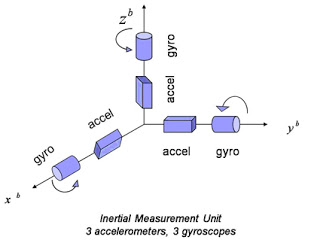
\includegraphics[height=0.7\linewidth]{Figures/imu_6dof.jpg}
  \captionof{figure}{Inertial Measurement Unit (IMU) with three orthogonal gyroscopes and accelerometer \cite{2021InertialTracking}.}
  \label{fig:IMU6DOF}
\end{minipage}%
\begin{minipage}{.5\textwidth}
  \centering
  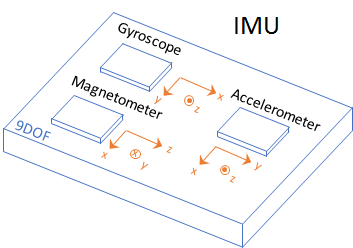
\includegraphics[height=0.7\linewidth]{Figures/imu_diagram.png}
  \captionof{figure}{Nine DoF IMU diagram \cite{2021ModelSimulink}}
  \label{fig:9DOFIMU}
\end{minipage}
\end{figure}


\noindent INS's accuracy depends on the IMU grades, with strategic IMU Grade as the most accurate with a positional error of 30-100 m/h \cite{El-Sheimy2020InertialTrends}. Due to its accuracy, size, and external dependency, INS has been used in a broad navigation and guidance system. Below are some of the most common application of modern INS.\\

\subsubsection{Aircraft Navigation}
INS is exceptionally well known in a long-range aircraft navigation system. INS's basis in aircraft navigation is dead-reckoning, where initialisation of a point in space is required before its use. INS allows calculation of its position and velocity based on acceleration measurement over time \cite{El-Sheimy2020InertialTrends}\cite{Loewy2003AircraftAvionics}. The history of INS was first deployed solely for submarines and was too heavy for flying machines. With the rapid improvement of size and weight reduction, INS is widely used in modern aircraft.\\

\begin{figure}[!ht]
\begin{center}
%    
  \begin{subfigure}[b]{0.55\textwidth}
    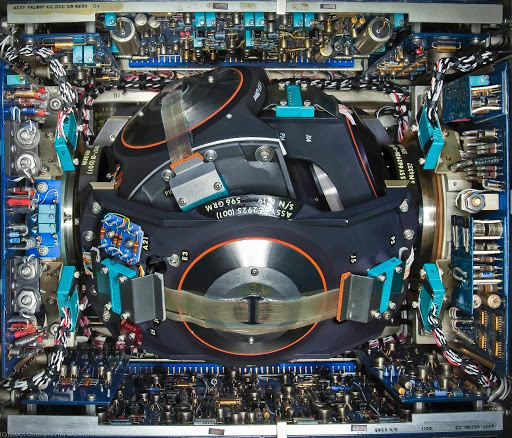
\includegraphics[height=6cm]{Figures/INS_Concorde.jpg}
  \end{subfigure}
%
  \begin{subfigure}[b]{0.35\textwidth}
    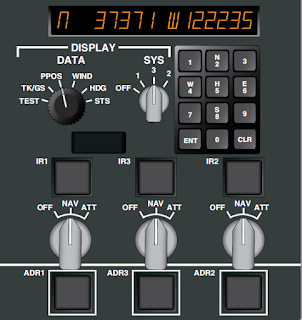
\includegraphics[height=6cm]{Figures/INS-IRS_InterfacePanel.png}
  \end{subfigure}
%  
  \caption{Physical INS System Used in Concorde (left) and Airbus INS Interface Panel Illustration (right).}
    \label{fig:concordeINS}
\end{center}
\end{figure}

\noindent INS was a giant leap in aircraft navigation. Around the 1960s to 1990s, navigation reliability was challenged for an international flight around a higher earth latitude \cite{Anonymous1964InertialNavigation}. The higher earth's latitude is the minimum region of compass accuracy and ground-based navigation aids (tower, etc.), making the navigation system unreliable. At this time, independent navigation was needed to overcome the challenge, and INS was the solution.\\

\noindent Despite its accuracy and independence, INS build its error over its usage time. For instance, a tactical grade INS gain positional error up to 20 nautical miles per hour with gyroscope drift up to 10 deg per hour, which is not reliable for long-range navigation use. Therefore, in a modern navigation system, integrating another type of navigation system (such as GPS) is proven to aid these issues.\\

\subsubsection{Submarine Navigation}
Before the INS became small and light, INS was broadly used for the submarine navigation system known as Ship Inertial Navigation System (SINS) \cite{NATOSINS}. The same concept applies where INS uses acceleration measurement to calculate the submarines' latitude, longitude, heading, and altitude, given the initial referencing point.  One example of INS application in a submarine is U.S.S Alabama, where INS is integrated vis Central Navigation Computer (CNC) with TRANSIT, LORAN-C, and SONAR for its overall navigation purposes \cite{HowNavigation}. Figure \ref{fig:USS_INS} shows the illustration of the U.S.S Alabama navigation system..\\

\noindent It is essential for a military submersible embeds an INS without any dependency on any other navigation aid. However, submarine design's objective is to travel in stealth mode where navigation which transmits waves such as GPS and sonar are not allowed \cite{Rogobete2018UsingPositioning}. For a long-range movement, the INS alone could build an error, and another navigation aid is required. To overcome this challenge, a Kalman filter with a Second Gradient of Gravity Field (SGG) sensor must allow continuous correction, which improves navigation accuracy and minimises INS drift. A simplified diagram of these schemes is shown in figure \ref{fig:INS_KALMAN}.\\

\noindent It is worth to be noted that in modern development, INS applications with other navigational aid is also used in autonomous submerged vehicles for research and military purposes.

\begin{figure}[!ht]
    \centering
    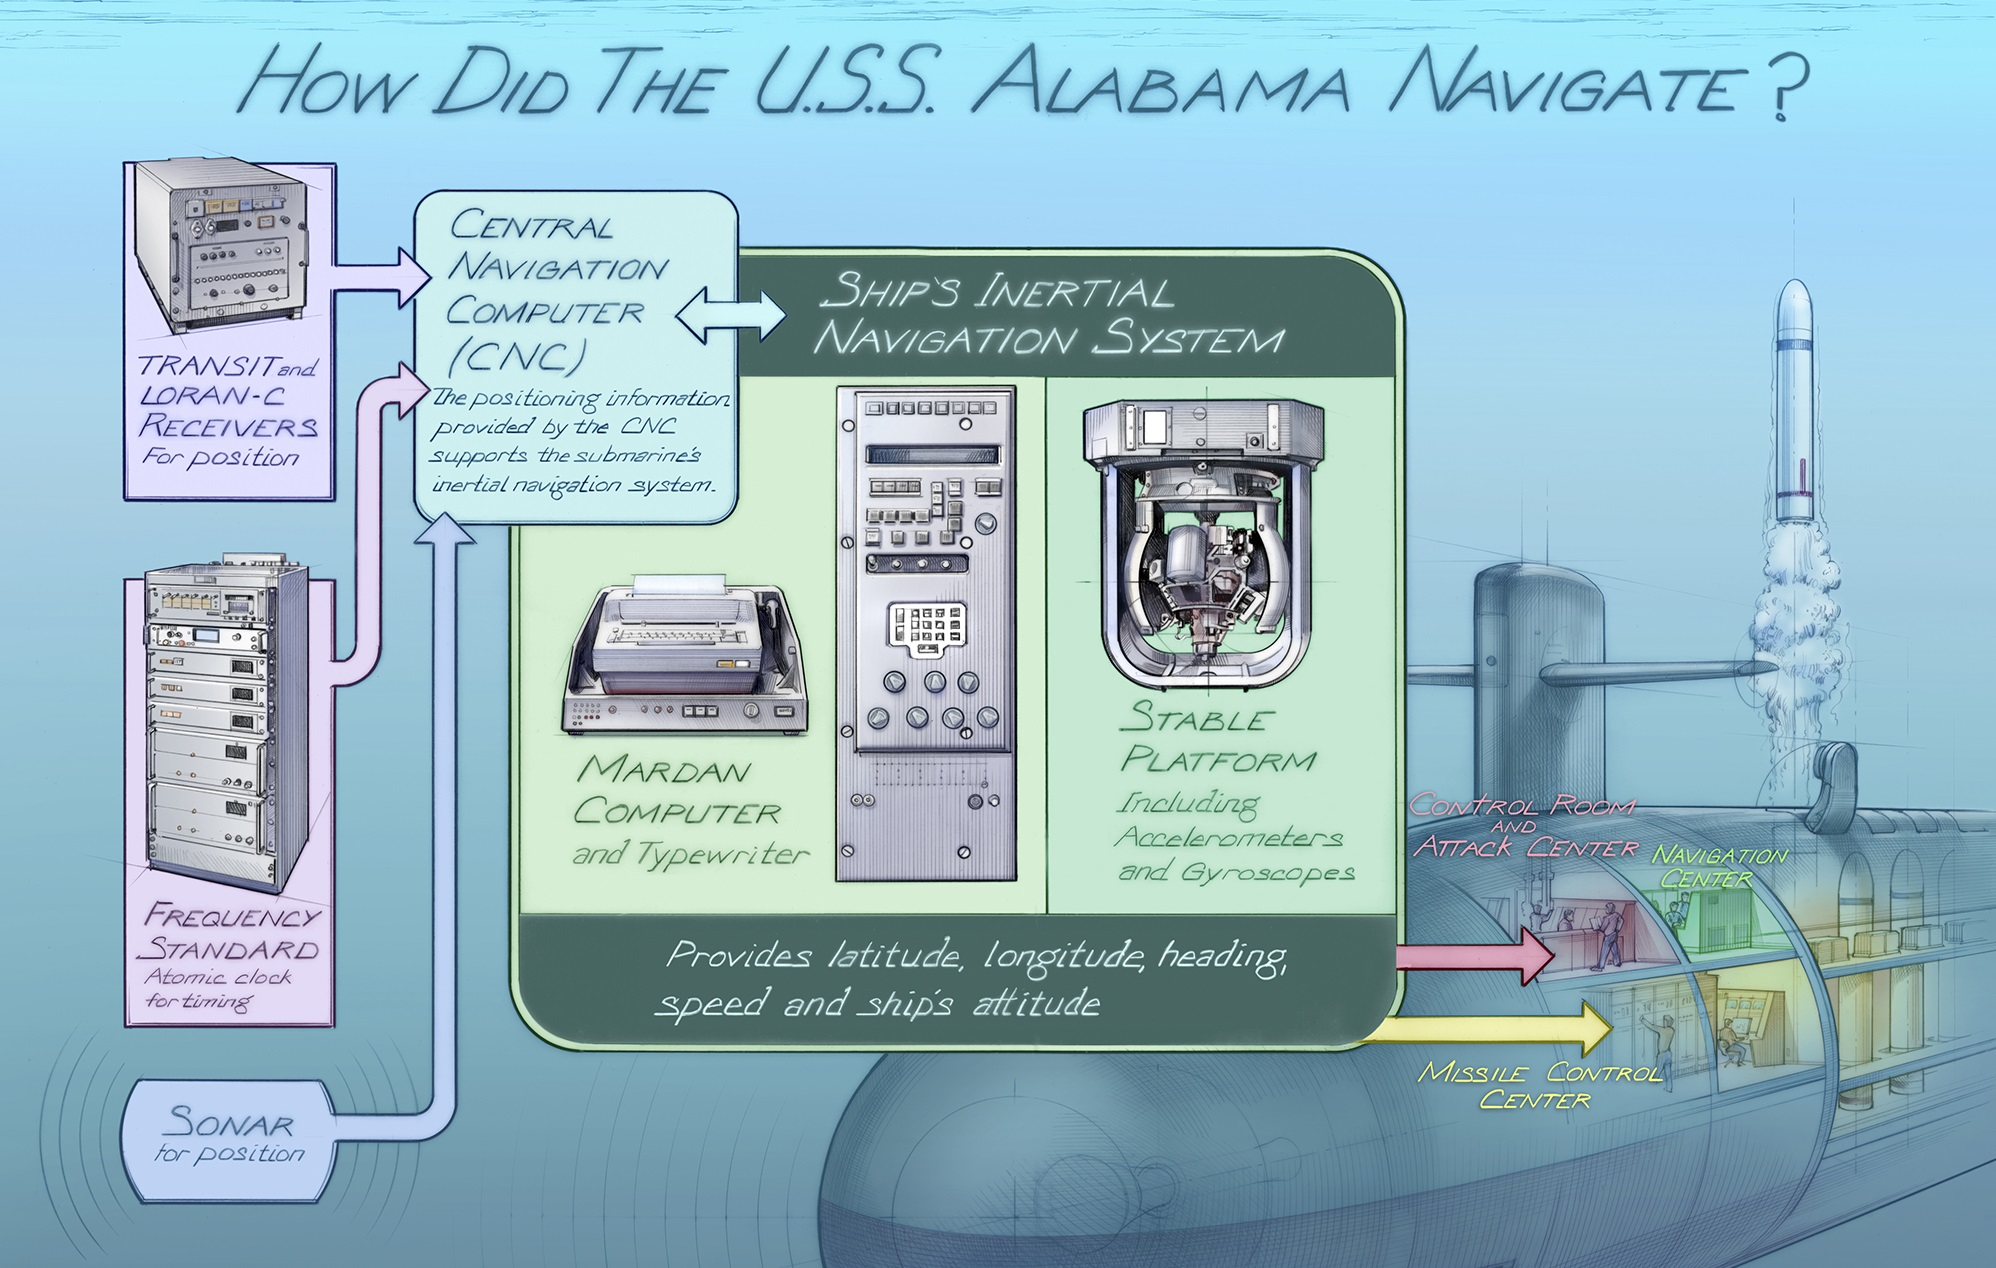
\includegraphics[scale=0.5]{Figures/USS_Alabama_INS.jpg}
    \caption{Simplified diagram of USS Alabama INS Navigation System \cite{HowNavigation}. }
    \label{fig:USS_INS}
    \vspace{2mm}
    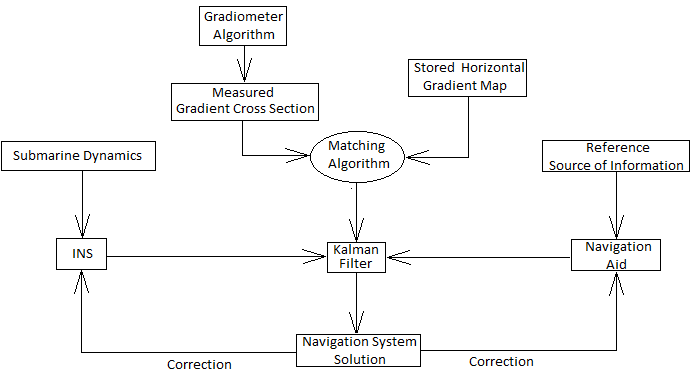
\includegraphics[scale=0.7]{Figures/INS Scheme KALMAN filter.png}
    \caption{INS Diagram correlated to Kalman filter with navigation aid and matching algorithm to improve drift correction \cite{Rogobete2018UsingPositioning}. }
    \label{fig:INS_KALMAN}
\end{figure}
\vspace{3cm}

\subsection{Enhanced Long Range Navigation (E-LORAN)}

%definition, basic system, difference between normal loran
Enhanced Long Range Navigation (E-LORAN) is a low-frequency navigation system which internationally standardised for positioning, navigation, and timing (PNT) \cite{EnhancedApril}\cite{InternationalLORANAssociation2007EnhancedApril}. The accuracy, integrity, and continuity of its performance makes it as reliable for various non-precision applications, such as; maritime, telecommunications, land navigation, etc. \\

\noindent eLoran was built with the foundation of its predecessor Loran-C, with the addition of a transmitted signal data channel which allows corrections, warnings, and signal integrity to its applications \cite{EnhancedApril}. Contrary to the Global Navigation Satellite System (GNSS), the eLoran system is independent, which has more excellent resistance to signal-jamming, and reception limitation \cite{Anonymous2009LORANELORAN}. It is also considered to be an alternative, part of an integrated system or backup to GNSS \cite{Son2020ELoran:Areas}. Figure \ref{fig:ELORAN_Ill} shows a simplified illustration of the eLoran system.

\begin{figure}[!ht]
    \centering
    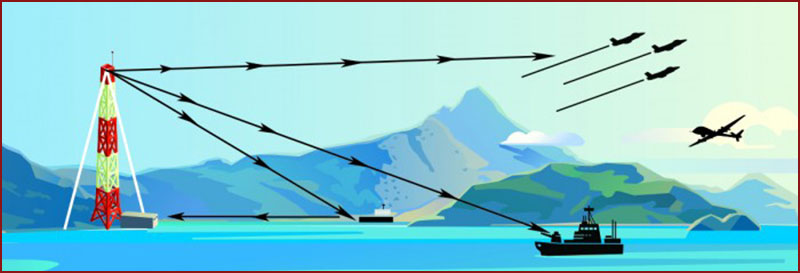
\includegraphics[scale = 0.5]{Figures/ELORAN_Ilustration.jpg}
    \caption{Simplified illustration of eLORAN system \cite{Anonymous2009LORANELORAN}}
    \label{fig:ELORAN_Ill}
\end{figure}
%
\subsubsection{Maritime Navigation}
The continuous growth of the world's shipping industry is expected to be large, demanding the requirements on a reliable, safe, and economic navigation system is high \cite{2004TheVision}. Maritime navigation system required accurate position and timing data, which principally generated from GNSS. However, GNSS solely can not provide constant availability and range due to its vulnerability. Therefore, integrating GNSS with eLoran is a safe yet redundant solution to deliver a high-range and safe navigation system \cite{InternationalLORANAssociation2007EnhancedApril}. To improve system accuracy and reduce time drifting, application service providers could also be integrated into the maritime service to generate specific application, such as; eLoran correction and signal propagation map. Figure \ref{fig:eloranmaritimeapp} below shows the diagram of application service provider integration to maritime service provision.\\

\begin{figure}[!ht]
    \centering
    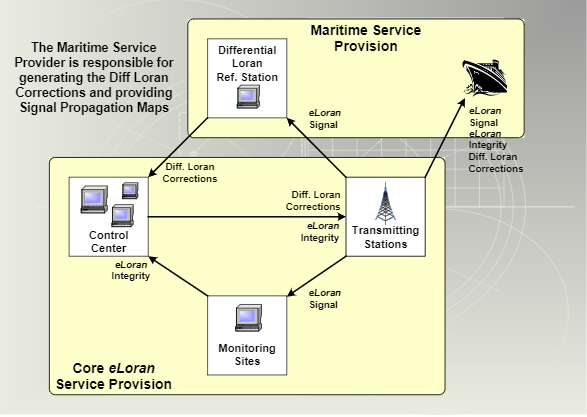
\includegraphics[scale=0.7]{Figures/ELORAN_maritime_app.PNG}
    \caption{Integrated eLoran Service to Maritime service provision \cite{InternationalLORANAssociation2007EnhancedApril}.}
    \label{fig:eloranmaritimeapp}
\end{figure}

\noindent For maritime application, a well-configured eLoran system can achieve 10 m with 95\% accuracy within 30-km field coverage, which follows the International Maritime Organisation (IMO) requirements for harbour and coastal operations, such as; harbour entrance/approach and coastal navigation \cite{SharedTutorial}\cite{Son2020ELoran:Areas}\cite{SafarAIONS}. Figure \ref{fig:eloranblanked} shows eLoran accuracy contour, which suggests 10-m positioning accuracy around most of the UK's coastal water and blanked pulse of one of the UK's eLoran station (Anthron).\\

\begin{figure}[!ht]
\begin{center}
%    
  \begin{subfigure}[b]{0.4\textwidth}
    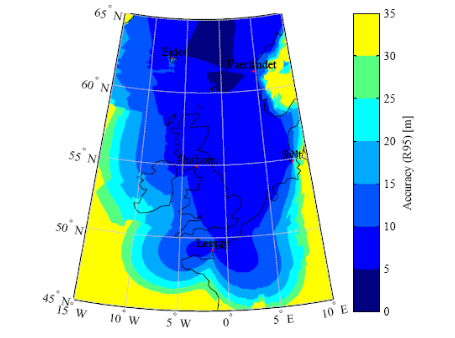
\includegraphics[height=5.3cm]{Figures/ELORAN_maritime_contour_UK.PNG}
  \end{subfigure}
%
  \begin{subfigure}[b]{0.5\textwidth}
    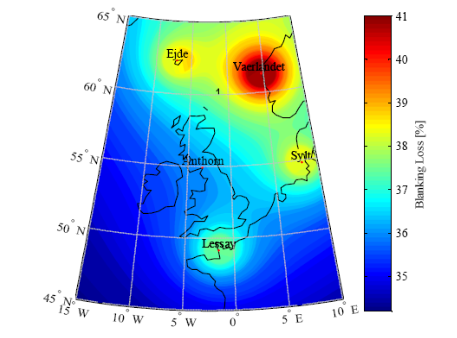
\includegraphics[height=5.3cm]{Figures/ELORAN_blanking_percentage.PNG}
  \end{subfigure}
%  
  \caption{Repeatable eLoran accuracy contour in the UK and Europe area with 95\% accuracy (left) and Blanked Pulse percentage of Anthorn station in 91 km ionosphere height (right) \cite{SafarAIONS}.}
    \label{fig:eloranblanked}
\end{center}
\end{figure}

\subsubsection{Aircraft Navigation \& Backup to GNSS}
eLoran successor, Loran-C is one of the approved navigation systems by the Federal Aviation Administration (FAA). In aviation application, the service is used to navigate and support its operation in departure, route, approach, and landing \cite{InternationalLORANAssociation2007EnhancedApril}\cite{BartoneH-fieldApplications}. To support three flight phase, the navigation system has to meet the Required Navigation Performance RNP 0.3 shown in table \ref{table:1}.\\

\begin{table}[h!]
\centering
\caption{Required Navigation Performance 0.3 (RNP 0.3).}
\begin{tabular}{||c c c c||} 
 \hline
Horizontal Accuracy & Availability & integrity & Continuity \\ [0.5ex] 
 \hline\hline
556 meters & 0.999-0.9999 & 1E-7 per hour & 0.999-0.9999 \\ [1ex]
 \hline
\end{tabular}
\label{table:1}
\end{table}

\noindent To fulfil the requirement, Signal Propagation Correction has to be issued for every airport and applied in real-time for each phase to maintain its accuracy. The crucial requirements in using eLoran is its integrity; from the table, it indicated that the probability of the system producing hazardous error has to be less than 1: 10,000,000 per hour \cite{InternationalLORANAssociation2007EnhancedApril}. eLoran has been demonstrated to be able to fulfil all the requirements and allow gate-to-gate navigation when GNSS disrupted \cite{InternationalLORANAssociation2007EnhancedApril}\cite{Narins2014TheBoard}.\\

\vspace{3mm}
\begin{figure}[!ht]
\begin{center}
%    
  \begin{subfigure}[b]{0.45\textwidth}
    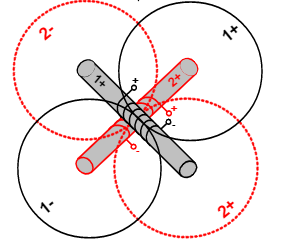
\includegraphics[height=5cm]{Figures/ELORAN_hfield_conf.PNG}
  \end{subfigure}
  %
  \begin{subfigure}[b]{0.5\textwidth}
    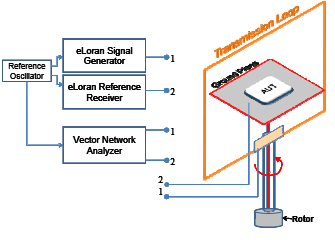
\includegraphics[height=5cm]{Figures/ELORAN_hfield__antenna_component.PNG}
  \end{subfigure}
%  
  \caption{Dual loop configuration of H-Field antenna (left) and H-Field eLoran Antenna Component test configuration (right) \cite{BartoneH-fieldApplications}.}
    \label{fig:hloop antenna}
\end{center}
\end{figure}
\vspace{3mm}

\noindent In a recent development, the usage of H-field or magnetic loop antenna for eLoran has been demonstrated to fulfil the requirements for the purposes of Minimum Operation Performance Specification \cite{Anonymous2016ELoranLight}. The primary issue form the previous generation Loran-C and E-field antenna is the signal noise caused by the electrical potential from the airframe and its surroundings (particularly in snow and rain); this disruption is also known as P-Static \cite{BartoneH-fieldApplications}.\\

\noindent Economically, eLoran system allows a potential to decrease land infrastructure, also enable Communication, Navigation, and Surveillance (CNS) function to transfer to digital communications \cite{InternationalLORANAssociation2007EnhancedApril}.\\